\documentclass{article}


\usepackage{parskip,wrapfig,graphicx}
\usepackage{hyperref}
\usepackage{fullpage}

\hypersetup{
    colorlinks,
    citecolor=black,
    filecolor=black,
    linkcolor=black,
    urlcolor=black
}




\title{Curta Type 3DP Build Manual}
\date{}

\begin{document}
\maketitle

\tableofcontents

\newpage

\section{Introduction}
This build manual is an attempt to describe the detailed and extensively manual process by which
I build my 3D printed Curta Calculators.


\section{Change Log}

\section{Safety Warning}


\section{Tools and Parts}

\section{A Note About Fitting Parts}

\section{Preparing and Painting External Facing Parts}


\section{Preparing Main Casting and Bearing Plate}
\subsection{Parts Required}

\subsection{Tools Required}

\subsection{Process}

\subsubsection{Bearing Plate Diagram (from the bottom side)}



\newpage
\section{Step Drum and Bearing Plate}

\subsection{Parts Required}

\begin{table}[h!]
 \centering
 \begin{tabular}{clc}
    Part Number & Part Name & Quantity (if $>1$) \\ \hline
     13 & Step Drum Lower or Step Drum (with main axle) & \\
     45 & Step Drum Upper Or Main Axle Bottom & \\
     78 & Step Drum Pins & 3 \\
     49 & Anti-Rotation plate (called Anti-Reversal in BoM) & \\
     57 & Bearing Plate & 
   %  33 & Tens Bell & 
 \end{tabular}
\end{table}

\subsection{Tools Required}

\begin{itemize}
 \item Hex driver or screwdriver (depending on the type of bolts you have)
 \item PTFE spray lubricant
 \item Files
 \item Sandpaper
 \item Superglue (cyanoacrylic)
\end{itemize}




\subsection{Process}
If you opted for printing the step drum as one piece, fit the main axle bottom into the base of the
step drum. This should be a snug fit with the keys matching up inside the step drum preventing any
rotation of the bottom of the axle relative to the step drum.


\begin{wrapfigure}{r}{.45\textwidth}
 \centering
 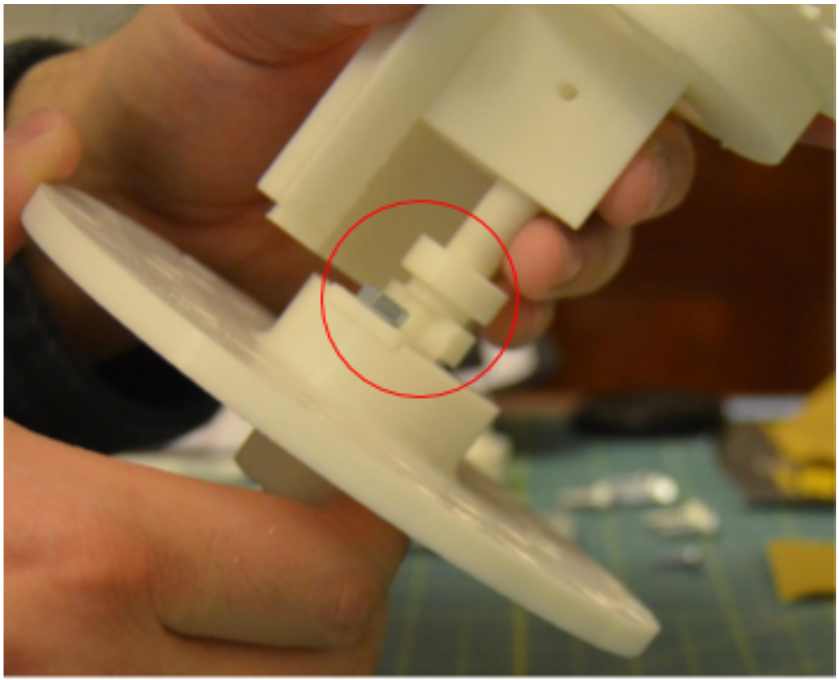
\includegraphics[width=.4\textwidth]{images/anti-rotation-collar.png}
 \caption{Alignment of the anti-rotation collar to the step drum}
\end{wrapfigure}

If you opted for printing the step drum in two pieces, fit the three pins into the lower piece of 
the step drum and super them into place. Once that has dried, add super glue to the pins of the lower
step drum and pres the upper half of the step drum onto the pins to combine the upper and lower
portions of the step drum into one piece.




The flat portion of the anti-rotation collar on the base of the axle needs to align with the right
side of the step drum when the toothed face of the step drum is facing you. This ensures that
the Curta will not switch between addition and subtraction when it is mid-rotation.



Now slide the step drum into the center of the bearing plate. The step drum should spin smoothly.
If it does not, file and sand it down until it does. Use some PTFE spray lubricant on the shaft and
the bearing plate. Do not allow the lubricant to reach the teeth of the step drum, but do allow it
to cover the anti-rotation collar. The fit should allow the step drum to spin freely. If you have to
sand further after spraying the lubricant, you will need to respray the parts that have already been
sanded.

Place the anti-rotation plate on the recessed portion of the bearing plate near the center. Turn the
step drum until the anti-rotation plate aligns with the collar and then slide the anti-rotation
plate to meet the flat portion of the anti-rotation collar. Test this fit to check that the plate
fits in the slots in the collar and that the step drum still moves freely. Sand and file as necessary
to make that happen. The step drum may need to slide up or down to align the plate with the middle 
section of the collar to get it in the correct position.

Now use a 10mm M5 bolt to secure the anti-rotation plate ensuring that it stays press against the
ant-rotation collar. If you need to, you can put a driver through the hole at the top of the step
drum to reach the bolt. I used plier for this since I had a hex bolt. \textbf{Do not over tighten
any of the screws or nuts in this build. If you strip the plastic the part will need to be reprinted}.
Fasteners should be tight, but don't crank down too much. If it will not stay as secure as you need,
use removeable threadlock.

Finally, double-check that you can still rotate the step drum smoothly and that the step drum can
switch between the raised (subtraction) position and the lowered (addition) position easily. If not,
you may need to file the anti-rotation plate or the collar some more and re-lubricate.



\newpage

\section{Tens Bell and Main Casting}

\subsection{Parts Required}
\begin{table}[h!]
	\centering
	\begin{tabular}{clc}
		Part Number & Part Name & Quantity (if $>1$) \\ \hline
		33 & Tens Bell & \\
		39 & Tens Bell c-clip & \\
		40 & Tens Bell spring & \\
		48 & Retaining fing for Tens Bell & \\
		56 & Main Casting (main body in BoM) & \\
		26 & Support Columns (Frame Support in BoM) & 3 
	\end{tabular}
\end{table}


\subsection{Tools Required}

\subsection{Process}


\newpage
\section{Springs for Zero Positioning Lever and Anti-Reversal Pawl}
\subsection{Parts Required}
\begin{table}[h!]
	\centering
	\begin{tabular}{clc}
		Part Number & Part Name & Quantity (if $>1$) \\ \hline
		- & 0.6mm Music Wire (0.024in) & \\
		- & 1.1mm Music Wire (0.043in) & 
	\end{tabular}
\end{table}



\subsection{Tools Required}

\subsection{Process}



\newpage
\section{Zero Positioning Disk}
\subsection{Parts Required}

\begin{table}[h!]
	\centering
	\begin{tabular}{clc}
		Part Number & Part Name & Quantity (if $>1$) \\ \hline
		27 & Zero Positioning Disc & \\
		67 & Zero Positioning Disc Lever & \\
		25 & Zero Positioning Disc Roller & \\
		66 & Anti Reversal Pawl (Reverse Rotation Prevention Pawl) & \\
		77 & Anti-Reversal Pawl Bolt Sleeve & \\
		76 & Zero Positioning Lever Bolt Sleeve & \\
		74 & Zero Positioning Disc Clip (Zero Positioning Plate Securing Spring) & \\
		71 & Main Axle Pin for Zero Positioning Disc & \\ \hline \hline
		- & Anti-Reversal Pawl Spring & \\
		- & Zero Positioning Lever Spring & \\ \hline \hline
		- & M5 hex head 10mm & 1 \\
		- & M5 hex head 20mm & 1 \\
		- & M5 hex head 30mm & 1 \\
		- & M5 nut & 2
	\end{tabular}
\end{table}

\subsection{Tools Required}

\subsection{Process}



\newpage
\section{Main Casting and Bearing Plate}
\subsection{Parts Required}
\begin{table}[h!]
	\centering
	\begin{tabular}{clc}
		Part Number & Part Name & Quantity (if $>1$) \\ \hline
		- & Assembled Main Casting and Tens Bell with Support Columns & \\
		- & Assembled Bearing Plate, Main Axle, and Step Drum & \\ \hline \hline
		- & M4 nuts & 3
	\end{tabular}
\end{table}



\subsection{Tools Required}

\subsection{Process}


\newpage
\section{Transmission Shafts}
\subsection{Parts Required}
\begin{table}[h!]
	\centering
	\begin{tabular}{clc}
		Part Number & Part Name & Quantity (if $>1$) \\ \hline
		6 & Double Transmission Gear &  \\
		7 & Standard Transmission Gear & 15 \\
		8 & Lockout &  \\
		9 & Triple Transmission Gear & \\
		10 & Tall Lockout & \\
		11 & Lockout with Transmission Gear & 15 \\
		28 & Ones Results Transmission Shaft & \\
		29 & Ones Turns Transmission Shaft & \\
		30 & Transmission Shaft & 12 \\
		31 & 9, 10, 11 Digits Transmission Shaft & 3 \\
		59 & Transmission Lock Ring (Cover Ring) & \\ \hline \hline
		- & M3 10mm Screws & 3
	\end{tabular}
\end{table}

\subsection{Tools Required}

\subsection{Process}


\newpage
\section{Reversing Lever}
\subsection{Parts Required}
\begin{table}[h!]
	\centering
	\begin{tabular}{clc}
		Part Number & Part Name & Quantity (if $>1$) \\ \hline
		20 & Upper Reversing Lever Spacer & \\
		21 & Lower Reversing Lever Spacer & \\
		22 & Reversing Lever & \\
		23 & Reversing Lever Shaft & \\ \hline \hline
		- & M4 Nut & 1
	\end{tabular}
\end{table}


\subsection{Tools Required}

\subsection{Process}

\newpage
\section{Carry Levers}
\subsection{Parts Required}
\begin{table}[h!]
	\centering
	\begin{tabular}{clc}
		Part Number & Part Name & Quantity (if $>1$) \\ \hline
		37 & Results Carry Levers (Tens Slider for Results) & 10 \\
		38 & Turns Counter Carry Lever (Tens Slider for Turns Counter) & 5 \\
		68 & Carry Lever Bearings (Tens Slide Bearing) & 15 \\ \hline \hline
		- & 0.6mm Music Wire & \\
		- & 16mm M4 Screws & 25
	\end{tabular}
\end{table}

\subsection{Tools Required}

\subsection{Process}


\newpage
\section{Selector Shafts}
\subsection{Parts Required}
\begin{table}[h!]
	\centering
	\begin{tabular}{clc}
		Part Number & Part Name & Quantity (if $>1$) \\ \hline
		1 & Selector Shaft (Selector Shaft Bottom) & 8 \\
		2 & Selector Shaft Top & 8 \\
		4 & Selector Shaft Bearing & 8 \\
		65 & Selector Knob & 8 \\
		63 & Selector Shaft Guide Screw (Digit Selector Screw) & 8 \\
		19 & Selector Shaft Bearing Cover Plates (Setting Axle Holding Plate) & 2 \\ \hline \hline 
		- & Cheap Ball Point Pen Springs & 8 \\
		- & 5mm Ball Bearings & 8 \\
		- & M4 10 mm Screws & 4
	\end{tabular}
\end{table}


\subsection{Tools Required}

\subsection{Process}


\newpage
\section{Collar and Lower Housing}
\subsection{Parts Required}
\begin{table}[h!]
	\centering
	\begin{tabular}{clc}
		Part Number & Part Name & Quantity (if $>1$) \\ \hline
		64 & Curta Collar (Upper Outer Sleeve) & \\
		52 & Lower Housing & \\
		69 & Position Markers & 5 \\ \hline \hline
		13 & Position Marker Spring ($0.4\times3\times5$mm spring) & 5 \\
		14 & 3mm Position Marker Ball Bearings & 5 \\
		11 & M3 10mm Screws & 3
	\end{tabular}
\end{table}

\subsection{Tools Required}

\subsection{Process}


\newpage
\section{Carriage Casting Preparation}
\subsection{Parts Required}
\begin{table}[h!]
	\centering
	\begin{tabular}{clc}
		Part Number & Part Name & Quantity (if $>1$) \\ \hline
		14 & Carriage Casting (Counter Body) & \\
		15 & Counter Body Stop Pin & \\
		16 & Counter Body Spider Spring Pin & 2 \\
		53 & Clearing Stop Pin Sleeve & \\
		70 & Digits Axle & 17 \\ \hline \hline
		12 & 6mm Ball Bearing & 1
	\end{tabular}
\end{table}

\subsection{Tools Required}

\subsection{Process}



\newpage
\section{Results Dials}
\subsection{Parts Required}

\begin{table}[h!]
	\centering
	\begin{tabular}{clc}
		Part Number & Part Name & Quantity (if $>1$) \\ \hline
		43 & Results Dial Type 2 & 13 \\
		44 & Results Dial Type 1 & 4 \\
		60 & Half Carry Pins (Number roll carry pin half) & 8\\
		61 & Full Carry Pins (Number roll carry pin full) & 7
	\end{tabular}
\end{table}

\subsection{Tools Required}

\subsection{Process}


\newpage
\section{Carriage Cage and Upper Housing}
\subsection{Parts Required}
\begin{table}[h!]
	\centering
	\begin{tabular}{clc}
		Part Number & Part Name & Quantity (if $>1$) \\ \hline
		- & Carriage with Dial Axles and Dials & \\
		55 & Carriage Cage (Digits Cover) & \\
		36 & Upper Housing & \\
		73 & Upper Housing Pin (Carriage Pin) & 
	\end{tabular}
\end{table}

\subsection{Tools Required}

\subsection{Process}


\newpage
\section{Bearings and Spider Spring}
\subsection{Parts Required}
\begin{table}[h!]
	\centering
	\begin{tabular}{clc}
		Part Number & Part Name & Quantity (if $>1$) \\ \hline
		 17 & Spider Spring & \\ 
		 46 & Counter Ring Washer & \\ \hline \hline 
		 12 & 6m Ball Bearing & 17 
	\end{tabular}
\end{table}


\subsection{Tools Required}

\subsection{Process}


\newpage
\section{Clearing Cap}
\subsection{Parts Required}
\begin{table}[h!]
	\centering
	\begin{tabular}{clc}
		Part Number & Part Name & Quantity (if $>1$) \\ \hline
		24 & Clearing Ring Handle (Clearing Ring) & \\
		41 & Clearing Cap Teeth Spacer (Clearing Cap Tooth Segment Spacer) & \\
		42 & Clearing Cap Teeth & 2 \\
		47 & Clearing Cap (Clearing Cover) & \\
		58 & Clearing Cap Rivet (Clearing Ring Rivet) & 2 \\
		69 & Position Marker & 5 \\
		75 & Clearing Cap Stop Pin (Crank Pin) & \\ \hline \hline
		14 & 3mm Ball Bearing & 5 \\
		13 & Position Marker Spring ($0.4\times3\times5$mm spring) & 5 \\
		15 & Clearing Cap Stop Spring ($0.6\times5\times20$mm) &
	\end{tabular}
\end{table}

\subsection{Tools Required}

\subsection{Process}


\newpage
\section{Crank Collar}
\subsection{Parts Required}
\begin{table}[h!]
	\centering
	\begin{tabular}{clc}
		Part Number & Part Name & Quantity (if $>1$) \\ \hline
		 12 & Crank Collar Nut (Counter Sleeve Nut) & \\
		 18 & Crank Collar & \\
		 34 & Crank Collar Spacer Ring &\\
	\end{tabular}
\end{table}


\subsection{Tools Required}

\subsection{Process}

\newpage
\section{Carriage and Main Body}
\subsection{Parts Required}

\begin{table}[h!]
	\centering
	\begin{tabular}{clc}
		Part Number & Part Name & Quantity (if $>1$) \\ \hline
		 - & Completed Carriage & \\
		 - & Completed Curta Body & \\
		 35 & Main Crank Spring Sleeve & \\
		 51 & Spring Sleeve Clip & \\ \hline \hline
		 19 & Upper Carriage Spring ($1.8\times28\times40$mm) & \\
		 12 & 6mm Ball Bearing & 
	\end{tabular}
\end{table}


\subsection{Tools Required}

\subsection{Process}


\newpage
\section{Crank Handle}
\subsection{Parts Required}
\begin{table}[h!]
	\centering
	\begin{tabular}{clc}
		Part Number & Part Name & Quantity (if $>1$) \\ \hline
		- & Mostly Completed Curta & \\
		3 & Crank Handle Pin Screw & \\
		5 & Crank Handle & \\
		62 & Main Crank & \\
		72 & Main Axle Pin for Crank Handle
	\end{tabular}
\end{table}

\subsection{Tools Required}

\subsection{Process}


\end{document}






























